\documentclass{ximera}

%\usepackage{todonotes}

\newcommand{\todo}{}

\usepackage{esint} % for \oiint
\ifxake%%https://math.meta.stackexchange.com/questions/9973/how-do-you-render-a-closed-surface-double-integral
\renewcommand{\oiint}{{\large\bigcirc}\kern-1.56em\iint}
\fi


\graphicspath{
  {./}
  {ximeraTutorial/}
  {basicPhilosophy/}
  {functionsOfSeveralVariables/}
  {normalVectors/}
  {lagrangeMultipliers/}
  {vectorFields/}
  {greensTheorem/}
  {shapeOfThingsToCome/}
  {dotProducts/}
  {partialDerivativesAndTheGradientVector/}
  {../productAndQuotientRules/exercises/}
  {../normalVectors/exercisesParametricPlots/}
  {../continuityOfFunctionsOfSeveralVariables/exercises/}
  {../partialDerivativesAndTheGradientVector/exercises/}
  {../directionalDerivativeAndChainRule/exercises/}
  {../commonCoordinates/exercisesCylindricalCoordinates/}
  {../commonCoordinates/exercisesSphericalCoordinates/}
  {../greensTheorem/exercisesCurlAndLineIntegrals/}
  {../greensTheorem/exercisesDivergenceAndLineIntegrals/}
  {../shapeOfThingsToCome/exercisesDivergenceTheorem/}
  {../greensTheorem/}
  {../shapeOfThingsToCome/}
  {../separableDifferentialEquations/exercises/}
  {vectorFields/}
}

\newcommand{\mooculus}{\textsf{\textbf{MOOC}\textnormal{\textsf{ULUS}}}}

\usepackage{tkz-euclide}
\usepackage{tikz}
\usepackage{tikz-cd}
\usetikzlibrary{arrows}
\tikzset{>=stealth,commutative diagrams/.cd,
  arrow style=tikz,diagrams={>=stealth}} %% cool arrow head
\tikzset{shorten <>/.style={ shorten >=#1, shorten <=#1 } } %% allows shorter vectors

\usetikzlibrary{backgrounds} %% for boxes around graphs
\usetikzlibrary{shapes,positioning}  %% Clouds and stars
\usetikzlibrary{matrix} %% for matrix
\usepgfplotslibrary{polar} %% for polar plots
\usepgfplotslibrary{fillbetween} %% to shade area between curves in TikZ
%\usetkzobj{all}
\usepackage[makeroom]{cancel} %% for strike outs
%\usepackage{mathtools} %% for pretty underbrace % Breaks Ximera
%\usepackage{multicol}
\usepackage{pgffor} %% required for integral for loops



%% http://tex.stackexchange.com/questions/66490/drawing-a-tikz-arc-specifying-the-center
%% Draws beach ball
\tikzset{pics/carc/.style args={#1:#2:#3}{code={\draw[pic actions] (#1:#3) arc(#1:#2:#3);}}}



\usepackage{array}
\setlength{\extrarowheight}{+.1cm}
\newdimen\digitwidth
\settowidth\digitwidth{9}
\def\divrule#1#2{
\noalign{\moveright#1\digitwidth
\vbox{\hrule width#2\digitwidth}}}




% \newcommand{\RR}{\mathbb R}
% \newcommand{\R}{\mathbb R}
% \newcommand{\N}{\mathbb N}
% \newcommand{\Z}{\mathbb Z}

\newcommand{\sagemath}{\textsf{SageMath}}


%\renewcommand{\d}{\,d\!}
%\renewcommand{\d}{\mathop{}\!d}
%\newcommand{\dd}[2][]{\frac{\d #1}{\d #2}}
%\newcommand{\pp}[2][]{\frac{\partial #1}{\partial #2}}
% \renewcommand{\l}{\ell}
%\newcommand{\ddx}{\frac{d}{\d x}}

% \newcommand{\zeroOverZero}{\ensuremath{\boldsymbol{\tfrac{0}{0}}}}
%\newcommand{\inftyOverInfty}{\ensuremath{\boldsymbol{\tfrac{\infty}{\infty}}}}
%\newcommand{\zeroOverInfty}{\ensuremath{\boldsymbol{\tfrac{0}{\infty}}}}
%\newcommand{\zeroTimesInfty}{\ensuremath{\small\boldsymbol{0\cdot \infty}}}
%\newcommand{\inftyMinusInfty}{\ensuremath{\small\boldsymbol{\infty - \infty}}}
%\newcommand{\oneToInfty}{\ensuremath{\boldsymbol{1^\infty}}}
%\newcommand{\zeroToZero}{\ensuremath{\boldsymbol{0^0}}}
%\newcommand{\inftyToZero}{\ensuremath{\boldsymbol{\infty^0}}}



% \newcommand{\numOverZero}{\ensuremath{\boldsymbol{\tfrac{\#}{0}}}}
% \newcommand{\dfn}{\textbf}
% \newcommand{\unit}{\,\mathrm}
% \newcommand{\unit}{\mathop{}\!\mathrm}
% \newcommand{\eval}[1]{\bigg[ #1 \bigg]}
% \newcommand{\seq}[1]{\left( #1 \right)}
% \renewcommand{\epsilon}{\varepsilon}
% \renewcommand{\phi}{\varphi}


% \renewcommand{\iff}{\Leftrightarrow}

% \DeclareMathOperator{\arccot}{arccot}
% \DeclareMathOperator{\arcsec}{arcsec}
% \DeclareMathOperator{\arccsc}{arccsc}
% \DeclareMathOperator{\si}{Si}
% \DeclareMathOperator{\scal}{scal}
% \DeclareMathOperator{\sign}{sign}


%% \newcommand{\tightoverset}[2]{% for arrow vec
%%   \mathop{#2}\limits^{\vbox to -.5ex{\kern-0.75ex\hbox{$#1$}\vss}}}
% \newcommand{\arrowvec}[1]{{\overset{\rightharpoonup}{#1}}}
% \renewcommand{\vec}[1]{\arrowvec{\mathbf{#1}}}
% \renewcommand{\vec}[1]{{\overset{\boldsymbol{\rightharpoonup}}{\mathbf{#1}}}}

% \newcommand{\point}[1]{\left(#1\right)} %this allows \vector{ to be changed to \vector{ with a quick find and replace
% \newcommand{\pt}[1]{\mathbf{#1}} %this allows \vec{ to be changed to \vec{ with a quick find and replace
% \newcommand{\Lim}[2]{\lim_{\point{#1} \to \point{#2}}} %Bart, I changed this to point since I want to use it.  It runs through both of the exercise and exerciseE files in limits section, which is why it was in each document to start with.

% \DeclareMathOperator{\proj}{\mathbf{proj}}
% \newcommand{\veci}{{\boldsymbol{\hat{\imath}}}}
% \newcommand{\vecj}{{\boldsymbol{\hat{\jmath}}}}
% \newcommand{\veck}{{\boldsymbol{\hat{k}}}}
% \newcommand{\vecl}{\vec{\boldsymbol{\l}}}
% \newcommand{\uvec}[1]{\mathbf{\hat{#1}}}
% \newcommand{\utan}{\mathbf{\hat{t}}}
% \newcommand{\unormal}{\mathbf{\hat{n}}}
% \newcommand{\ubinormal}{\mathbf{\hat{b}}}

% \newcommand{\dotp}{\bullet}
% \newcommand{\cross}{\boldsymbol\times}
% \newcommand{\grad}{\boldsymbol\nabla}
% \newcommand{\divergence}{\grad\dotp}
% \newcommand{\curl}{\grad\cross}
%\DeclareMathOperator{\divergence}{divergence}
%\DeclareMathOperator{\curl}[1]{\grad\cross #1}
% \newcommand{\lto}{\mathop{\longrightarrow\,}\limits}

% \renewcommand{\bar}{\overline}

\colorlet{textColor}{black}
\colorlet{background}{white}
\colorlet{penColor}{blue!50!black} % Color of a curve in a plot
\colorlet{penColor2}{red!50!black}% Color of a curve in a plot
\colorlet{penColor3}{red!50!blue} % Color of a curve in a plot
\colorlet{penColor4}{green!50!black} % Color of a curve in a plot
\colorlet{penColor5}{orange!80!black} % Color of a curve in a plot
\colorlet{penColor6}{yellow!70!black} % Color of a curve in a plot
\colorlet{fill1}{penColor!20} % Color of fill in a plot
\colorlet{fill2}{penColor2!20} % Color of fill in a plot
\colorlet{fillp}{fill1} % Color of positive area
\colorlet{filln}{penColor2!20} % Color of negative area
\colorlet{fill3}{penColor3!20} % Fill
\colorlet{fill4}{penColor4!20} % Fill
\colorlet{fill5}{penColor5!20} % Fill
\colorlet{gridColor}{gray!50} % Color of grid in a plot

\newcommand{\surfaceColor}{violet}
\newcommand{\surfaceColorTwo}{redyellow}
\newcommand{\sliceColor}{greenyellow}




\pgfmathdeclarefunction{gauss}{2}{% gives gaussian
  \pgfmathparse{1/(#2*sqrt(2*pi))*exp(-((x-#1)^2)/(2*#2^2))}%
}


%%%%%%%%%%%%%
%% Vectors
%%%%%%%%%%%%%

%% Simple horiz vectors
\renewcommand{\vector}[1]{\left\langle #1\right\rangle}


%% %% Complex Horiz Vectors with angle brackets
%% \makeatletter
%% \renewcommand{\vector}[2][ , ]{\left\langle%
%%   \def\nextitem{\def\nextitem{#1}}%
%%   \@for \el:=#2\do{\nextitem\el}\right\rangle%
%% }
%% \makeatother

%% %% Vertical Vectors
%% \def\vector#1{\begin{bmatrix}\vecListA#1,,\end{bmatrix}}
%% \def\vecListA#1,{\if,#1,\else #1\cr \expandafter \vecListA \fi}

%%%%%%%%%%%%%
%% End of vectors
%%%%%%%%%%%%%

%\newcommand{\fullwidth}{}
%\newcommand{\normalwidth}{}



%% makes a snazzy t-chart for evaluating functions
%\newenvironment{tchart}{\rowcolors{2}{}{background!90!textColor}\array}{\endarray}

%%This is to help with formatting on future title pages.
\newenvironment{sectionOutcomes}{}{}



%% Flowchart stuff
%\tikzstyle{startstop} = [rectangle, rounded corners, minimum width=3cm, minimum height=1cm,text centered, draw=black]
%\tikzstyle{question} = [rectangle, minimum width=3cm, minimum height=1cm, text centered, draw=black]
%\tikzstyle{decision} = [trapezium, trapezium left angle=70, trapezium right angle=110, minimum width=3cm, minimum height=1cm, text centered, draw=black]
%\tikzstyle{question} = [rectangle, rounded corners, minimum width=3cm, minimum height=1cm,text centered, draw=black]
%\tikzstyle{process} = [rectangle, minimum width=3cm, minimum height=1cm, text centered, draw=black]
%\tikzstyle{decision} = [trapezium, trapezium left angle=70, trapezium right angle=110, minimum width=3cm, minimum height=1cm, text centered, draw=black]


\title{3 Views}

\begin{document}

\begin{abstract}
information
\end{abstract}
\maketitle




We now have three views of the same information.



\begin{itemize}
\item \textbf{\textcolor{purple!85!blue}{Geometry}} We have the Cartesian plane, which consists of points.  These points have locations described by rectangular coordinates. \\

\item \textbf{\textcolor{purple!85!blue}{Geometry}} We can describe these locations with polar (circular) coordinates. \\

\item \textbf{\textcolor{purple!85!blue}{Arithmetic}} We can now glue a layer of arthmetic over these same points with the Complex Numbers.
\end{itemize}


These are three ways to describe the same information.  The sit on top of each other and we choose which lens to look through.  This also allows us to quickly change lens.  We can begin thinking one way and then quickly change to a different perspective, where we might have better ideas. \\

We can begin with a geometric question, rephrase it in terms of arithmetic, apply some algebra, and then interpret back into geometry. \\

We can begin with an algebra question (like about functions), consider the graph, apply some geometry, and then interpret the results back into arithmetic.  \\




\subsection*{Rectangular Coordinates}

The location or position of a point can be described with left/right and up/down measurements from the origin, $(0,0)$, which are called \textit{coordinates}.  The first coordinate gives the horizontal measurement and the second coordinate gives the up/down measurement.  Our favorite names for these directions are $x$ and $y$. The coordinates are written as ordered pairs: $(x_0, y_0)$.

\textbf{Note:} $x_0$ and $y_0$ are specific values measured in the $x$ and $y$ directions. 


Distance, measurement, position, location, coordinates, and direction are all geometric information.  Left/Right and up/down are the directions forming rectangles, hence, we call these \textit{rectangular coordinates}.







\begin{image}
\begin{tikzpicture}
  \begin{axis}[
            domain=-10:10, ymax=10, xmax=10, ymin=-10, xmin=-10,
            axis lines =center, xlabel=$x$, ylabel=$y$,
            ytick={-10,-8,-6,-4,-2,2,4,6,8,10},
            xtick={-10,-8,-6,-4,-2,2,4,6,8,10},
            ticklabel style={font=\scriptsize},
            every axis y label/.style={at=(current axis.above origin),anchor=south},
            every axis x label/.style={at=(current axis.right of origin),anchor=west},
            axis on top
          ]
          
          \addplot[color=penColor,only marks,mark=*] coordinates{(7,5)}; 

          \addplot [line width=1, penColor, smooth,samples=100,domain=(-0.25:0.25)] ({7},{x});
          \addplot [line width=1, penColor, smooth,samples=100,domain=(-0.25:0.25)] ({x},{5});

          \node at (axis cs:7,-0.75) [penColor] {\scriptsize $A$};
          \node at (axis cs:-0.75,5) [penColor] {\scriptsize $B$};
          \node at (axis cs:8,4) [penColor] {\scriptsize $(A,B)$};



  %\addplot [draw=penColor,very thick,smooth,domain=(-9:0),<-] {0};
  %\addplot [draw=penColor,very thick,smooth,domain=(0:9),->] {1};
  %\addplot[color=penColor,only marks,mark=*] coordinates{(0,1)}; 
  %\addplot[color=penColor,fill=white,only marks,mark=*] coordinates{(0,0)}; 

    \end{axis}
\end{tikzpicture}
\end{image}








\begin{image}
\begin{tikzpicture}
  \begin{axis}[
            domain=-5:5, ymax=5, xmax=5, ymin=-5, xmin=-5,
            axis lines =center, xlabel=$x$, ylabel=$y$,
            ytick={-4,-2,2,4},
            xtick={-4,-2,2,4},
            ticklabel style={font=\scriptsize},
            every axis y label/.style={at=(current axis.above origin),anchor=south},
            every axis x label/.style={at=(current axis.right of origin),anchor=west},
            axis on top
          ]
          
          \addplot[color=penColor,only marks,mark=*] coordinates{(3.5,2.5)}; 

          \addplot [line width=1, penColor, smooth,samples=100,domain=(-0.25:0.25)] ({3.5},{x});
          \addplot [line width=1, penColor, smooth,samples=100,domain=(-0.25:0.25)] ({x},{2.5});

          \node at (axis cs:3.5,-0.75) [penColor] {\scriptsize $A$};
          \node at (axis cs:-0.75,2.5) [penColor] {\scriptsize $B$};
          \node at (axis cs:4,2) [penColor] {\scriptsize $(A,B)$};



  %\addplot [draw=penColor,very thick,smooth,domain=(-9:0),<-] {0};
  %\addplot [draw=penColor,very thick,smooth,domain=(0:9),->] {1};
  %\addplot[color=penColor,only marks,mark=*] coordinates{(0,1)}; 
  %\addplot[color=penColor,fill=white,only marks,mark=*] coordinates{(0,0)}; 

    \end{axis}
\end{tikzpicture}
\end{image}





The location of every point in the plane can be described using rectanglular coordinates.








\subsection*{Polar Coordinates}



The location or position of a point can be described with a different set of measurements, which are still called \textit{coordinates}.  In this new measurement system, the second coordinate gives the direction of the point. This coordinate is given as an angle measurement as measured counterclockwise from the positive direction of the horizontal axis (from the rectangular system). It is a rotational measurement.  The first coordinate is the radial measurement from the origin, $(0,0)$. Our favorite names for these directions are $r$ and $\theta$. These are written as ordered pairs: $(r_0, \theta_0)$.


Distance, measurement, position, location, coordinates, and direction are all geometric information.  Left/Right and up/down are the directions forming rectangles, hence, we call these \textit{rectangular coordinates}.








  \begin{image}
    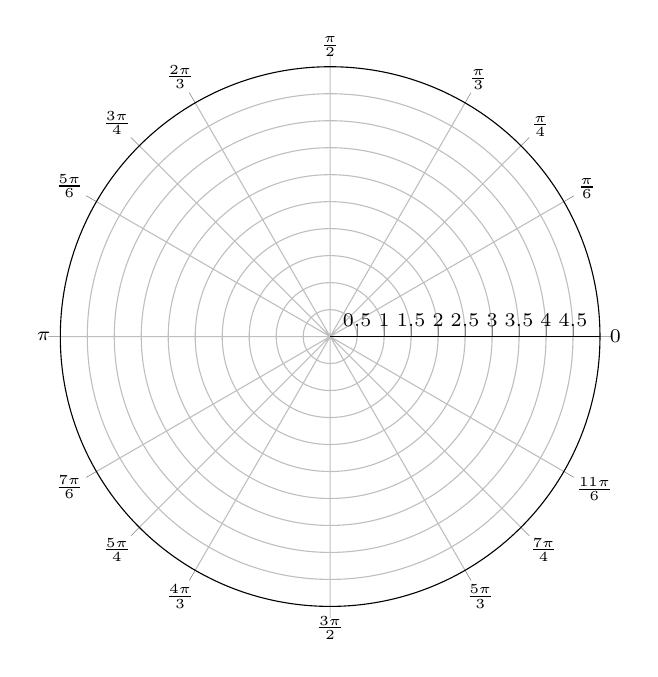
\begin{tikzpicture}
      \begin{polaraxis}[
          xmin=0,xmax=360, ymin=0,ymax=5,
          xtick={0,30,45,60,90,120,135,150,180,210,225,240,270,300,315,330,360}, style={font=\scriptsize},
          xticklabels={$0$,$\frac{\pi}{6}$,$\frac{\pi}{4}$,$\frac{\pi}{3}$,$\frac{\pi}{2}$,$\frac{2\pi}{3}$,$\frac{3\pi}{4}$,$\frac{5\pi}{6}$,$\pi$,$\frac{7\pi}{6}$,$\frac{5\pi}{4}$,$\frac{4\pi}{3}$,$\frac{3\pi}{2}$,$\frac{5\pi}{3}$,$\frac{7\pi}{4}$,$\frac{11\pi}{6}$,$2\pi$},
          ytick={.5,1,...,4.5},%yticklabels={},
        ]
        %\addplot+[draw=none, mark=none,penColor,domain=0:360,samples=100,smooth] {1};
      \end{polaraxis}
    \end{tikzpicture}
  \end{image}







































\begin{image}
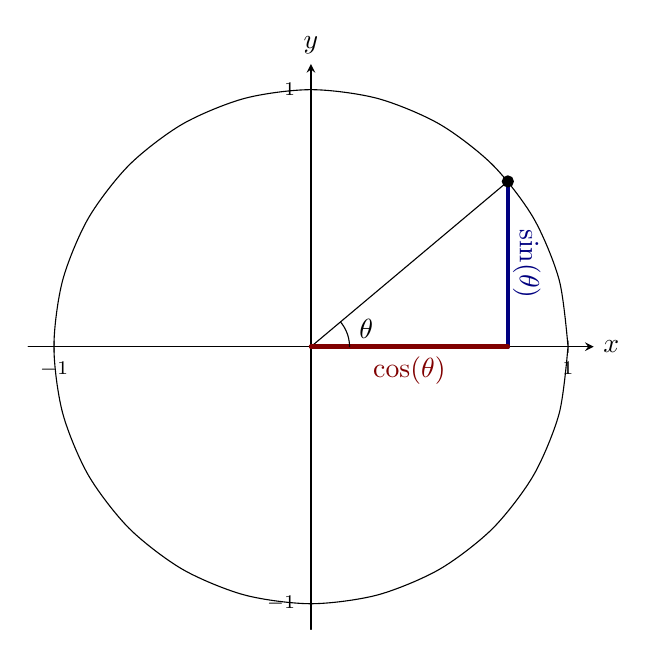
\begin{tikzpicture}[line cap=round]
  \begin{axis}[
            xmin=-1.1,xmax=1.1,ymin=-1.1,ymax=1.1,
            axis lines=center,
            width=4in,
            xtick={-1,1},
            ytick={-1,1},
            clip=false,
            unit vector ratio*=1 1 1,
            xlabel=$x$, ylabel=$y$,
            ticklabel style={font=\scriptsize},
            every axis y label/.style={at=(current axis.above origin),anchor=south},
            every axis x label/.style={at=(current axis.right of origin),anchor=west},
          ]        
          \addplot [smooth, domain=(0:360)] ({cos(x)},{sin(x)}); %% unit circle

          \addplot [textColor] plot coordinates {(0,0) (.766,.643)}; %% 40 degrees

          \addplot [ultra thick,penColor] plot coordinates {(.766,0) (.766,.643)}; %% 40 degrees
          \addplot [ultra thick,penColor2] plot coordinates {(0,0) (.766,0)}; %% 40 degrees
          
          %\addplot [ultra thick,penColor3] plot coordinates {(1,0) (1,.839)}; %% 40 degrees          

          \addplot [textColor,smooth, domain=(0:40)] ({.15*cos(x)},{.15*sin(x)});
          %\addplot [very thick,penColor] plot coordinates {(0,0) (.766,.643)}; %% sector
          %\addplot [very thick,penColor] plot coordinates {(0,0) (1,0)}; %% sector
          %\addplot [very thick, penColor, smooth, domain=(0:40)] ({cos(x)},{sin(x)}); %% sector
          \node at (axis cs:.15,.07) [anchor=west] {$\theta$};
          \node[penColor, rotate=-90] at (axis cs:.84,.322) {$\sin(\theta)$};
          \node[penColor2] at (axis cs:.383,0) [anchor=north] {$\cos(\theta)$};
          %\node[penColor3, rotate=-90] at (axis cs:1.06,.322) {$\tan(\theta)$};

          \addplot[color=black,fill=black,only marks,mark=*] coordinates{(0.766,0.643)}; 

        \end{axis}
\end{tikzpicture}
\end{image}














\subsection*{Arithmetic}






























\begin{center}
\textbf{\textcolor{green!50!black}{ooooo=-=-=-=-=-=-=-=-=-=-=-=-=ooOoo=-=-=-=-=-=-=-=-=-=-=-=-=ooooo}} \\

more examples can be found by following this link\\ \link[More Examples of Right Triangles]{https://ximera.osu.edu/csccmathematics/precalculus2/precalculus2/rightTriangles/examples/exampleList}

\end{center}




\end{document}

